\documentclass{report}
\usepackage[utf8]{vietnam}
\usepackage{amsmath}
\usepackage{setspace}
\usepackage{fancyhdr}
\usepackage{indentfirst}
\usepackage{amsmath}
\usepackage{amsfonts}
\usepackage{amssymb}
\usepackage{wrapfig}
\usepackage{multirow}
\usepackage{array}
\usepackage{color}
\usepackage{hyperref}
\usepackage{graphicx}
\usepackage{float}
\usepackage{flafter}
\usepackage{placeins} 
\usepackage{float} 
\usepackage{caption}
\usepackage{tocloft}
\usepackage{amsmath,amsxtra,amssymb,latexsym, amscd,amsthm}\usepackage[left=2.5cm,right=2.5cm,top=2.5cm,bottom=2.5cm]{geometry}
\newcommand\tab[1][1.25cm]{\hspace*{#1}}

\begin{document}
\begin{center}
	\pagenumbering{gobble}
	\fontsize{14}{20}\selectfont
	\textsc{TỔNG LIÊN ĐOÀN LAO ĐỘNG VIỆT NAM\\ 
		\textbf{TRƯỜNG ĐẠI HỌC TÔN ĐỨC THẮNG\\} 
		\textbf{KHOA CÔNG NGHỆ THÔNG TIN}}
	
	\vspace{0.08cm}
	\begin{figure}[htp]
		\begin{center}
			
\includegraphics[scale=1]{img/tdt.jpg}
		\end{center}
	\end{figure}
	
	\fontsize{15}{20}\selectfont\textbf{BÁO CÁO GIỮA KÌ MÔN\\ KIẾN TRÚC HƯỚNG DỊCH VỤ\\}
	
	\vspace{1.1cm}
	\fontsize{22}{20}\selectfont\textbf{PHÂN HỆ QUẢN LÝ ĐƠN HÀNG CỦA THỰC KHÁCH}
\end{center}
\vspace{2cm}
\begin{flushright}
	\setstretch{1.5}
	\fontsize{14}{20}\selectfont
	\textit{Người hướng dẫn}: \textbf{Thầy DƯƠNG HỮU PHÚC}\\
	
	\textit{Người thực hiện}:
	\textbf{PHẠM NGUYỄN HOÀNG QUÂN - 51900419}\\
	\textbf{NGUYỄN MINH PHƯỚC  - 51900770}\\
	\textbf{TRẦN HỮU NHẤT  - 519H0210}\\
	\textit{Khóa}: \textbf{23}\\
\end{flushright}
\vspace{4cm}
\begin{center}
	\fontsize{14}{20}\selectfont
	\textbf{THÀNH PHỐ HỒ CHÍ MINH, NĂM 2023}
\end{center}
\pagebreak
%------------------------------------------------------------
\begin{center}
	\pagenumbering{gobble}
	\fontsize{14}{20}\selectfont
	\textsc{TỔNG LIÊN ĐOÀN LAO ĐỘNG VIỆT NAM\\ 
		\textbf{TRƯỜNG ĐẠI HỌC TÔN ĐỨC THẮNG\\} 
		\textbf{KHOA CÔNG NGHỆ THÔNG TIN}}
	
	\vspace{0.08cm}
	\begin{figure}[htp]
		\begin{center}
			
\includegraphics[scale=1]{img/tdt.jpg}
		\end{center}
	\end{figure}
	
	\fontsize{15}{20}\selectfont\textbf{BÁO CÁO GIỮA KÌ MÔN\\ KIẾN TRÚC HƯỚNG DỊCH VỤ\\}
	
	\vspace{1.1cm}
	\fontsize{22}{20}\selectfont\textbf{PHÂN HỆ QUẢN LÝ ĐƠN HÀNG CỦA THỰC KHÁCH}
\end{center}
\vspace{2cm}
\begin{flushright}
	\setstretch{1.5}
	\fontsize{14}{20}\selectfont
	\textit{Người hướng dẫn}: \textbf{Thầy DƯƠNG HỮU PHÚC}\\
	
	\textit{Người thực hiện}:
	\textbf{PHẠM NGUYỄN HOÀNG QUÂN - 51900419}\\
	\textbf{NGUYỄN MINH PHƯỚC  - 51900770}\\
	\textbf{TRẦN HỮU NHẤT  - 519H0210}\\
	\textit{Khóa}: \textbf{23}\\
\end{flushright}
\vspace{4cm}
\begin{center}
	\fontsize{14}{20}\selectfont
	\textbf{THÀNH PHỐ HỒ CHÍ MINH, NĂM 2023}
\end{center}
\pagebreak
%------------------------------------------------------------
\pagestyle{fancy}
\fancyhf{}
\chead{\thepage}
\renewcommand{\headrulewidth}{0pt}
\begin{center}
	\pagenumbering{roman}\setcounter{page}{1}
	\fontsize{16}{20}\selectfont
	\textbf{LỜI CẢM ƠN\\} 
\end{center}
	\setstretch{1.5}
	\fontsize{13}{15}\selectfont
	\paragraph{}
	Để hoàn thành được bài tập lớn này, chúng em xin gửi đến Ban giám hiệu trường Đại Học Tôn Đức Thắng vì đã tạo điều kiện về cơ sở vật chất với hệ thống thư viện hiện đại, đa dạng các loại sách, tài liệu thuận lợi cho việc tìm kiếm, nghiên cứu thông tin.
	\paragraph{}
	Xin cám ơn các Thầy, các Cô ở Khoa Công Nghệ Thông Tin – Trường Đại Học Tôn Đức Thắng đã truyền đạt những tri thức quý báu của mình cho chúng em trong suốt quá trình học tập tại trường. Cách riêng để chúng em được tiếp cận với những kiến thức cần thiết cho đồ án cuối kì này, đó là nhờ sự giảng dạy tận tình, chi tiết của Thầy Dương Hữu Phúc.
	\paragraph{}
	Chúng em xin chân thành cảm ơn Thầy đã tận tâm hướng dẫn môn học này trong từng buổi học trên lớp, lẫn buổi học trực tuyến tại nhà với vốn kiến thức vô cùng quý báu ấy. Nếu không có sự hỗ trợ, giảng dạy của cô thì chúng em chắc không thể nào hoàn thiện được những kĩ năng về môn học này. Cùng với sự tiếp xúc lần đầu với đề tài tìm hiểu về hệ thống quản lý nội thất nên kiến thức và kinh nghiệm của chúng em vẫn còn khá hạn chế. Chính vì vậy, không thể nào tránh được những thiếu sót trong khi làm, chúng em mong nhân được nhiều sự bổ sung quý giá từ cô cũng như các bạn trong lớp để kiến thức của tụi em được cũng cố và hoàn thiện hơn.
	\paragraph{}
	Lời cuối cùng, chúng em xin kính chúc đến quý Thầy Cô thật nhiều sức khỏe, thành công và hạnh phúc.
\pagebreak	
%------------------------------------------------------------
%|							PAGE ii							|
%------------------------------------------------------------
\begin{center}
	\setstretch{1.0}
	\fontsize{16}{20}\selectfont
	\textbf{ĐỒ ÁN ĐƯỢC HOÀN THÀNH}\\
	\textbf{TẠI TRƯỜNG ĐẠI HỌC TÔN ĐỨC THẮNG\\} 
\end{center}
\setstretch{1.5}
\fontsize{13}{15}\selectfont
\paragraph{}
Tôi xin cam đoan đây là sản phẩm đồ án của riêng tôi / chúng tôi và được sự hướng dẫn của GV. Dương Hữu Phúc. Các nội dung nghiên cứu, kết quả trong đề tài này là trung thực và chưa công bố dưới bất kỳ hình thức nào trước đây. Những số liệu trong các bảng biểu phục vụ cho việc phân tích, nhận xét, đánh giá được chính tác giả thu thập từ các nguồn khác nhau có ghi rõ trong phần tài liệu tham khảo.
\paragraph{}
Ngoài ra, trong đồ án còn sử dụng một số nhận xét, đánh giá cũng như số liệu của các tác giả khác, cơ quan tổ chức khác đều có trích dẫn và chú thích nguồn gốc.
\paragraph{}
\textbf{Nếu phát hiện có bất kỳ sự gian lận nào tôi xin hoàn toàn chịu trách nhiệm về nội dung đồ án của mình.} Trường đại học Tôn Đức Thắng không liên quan đến những vi phạm tác quyền, bản quyền do tôi gây ra trong quá trình thực hiện (nếu có).
\begin{flushright}
	TP. Hồ Chí Minh, ngày \tab[1cm] tháng \tab[1cm] năm \tab[1cm]\tab \\
	\textit{Tác giả \tab\tab\tab\tab\tab\\
		(ký tên và ghi rõ họ tên)\tab[3cm] \\
		\vspace{1.5cm}
		Phạm Nguyễn Hoàng Quân\tab\quad \tab\quad\\
		\vspace{1.5cm}
		Nguyễn Minh Phước\tab\quad \tab\quad\\
		\vspace{1.5cm}
		Trần Hữu Nhất\tab\quad \tab\quad\\}
\end{flushright}
\pagebreak
%------------------------------------------------------------
\begin{center}
	\setstretch{1.0}
	\fontsize{16}{20}\selectfont
	\textbf{PHẦN NHẬN XÉT VÀ ĐÁNH GIÁ CỦA GIẢNG VIÊN}\\
\end{center}
\setstretch{1.5}
\fontsize{13}{14}\selectfont
\textbf{Phần xác nhận của GV hướng dẫn}\\
\rule{17cm}{1pt}\\
\rule{17cm}{1pt}\\
\rule{17cm}{1pt}\\
\rule{17cm}{1pt}\\
\rule{17cm}{1pt}\\
\rule{17cm}{1pt}\\
\rule{17cm}{1pt}\\
\begin{flushright}
	TP. Hồ Chí Minh, ngày \tab[1cm] tháng \tab[1cm] năm \tab[1cm]\tab \\
	(ký tên và ghi rõ họ tên)\tab[2cm] \\
	\vspace{2cm}
\end{flushright}
\setstretch{1.5}
\fontsize{13}{14}\selectfont
\textbf{Phần đánh giá của GV chấm bài}\\
\rule{17cm}{1pt}\\
\rule{17cm}{1pt}\\
\rule{17cm}{1pt}\\
\rule{17cm}{1pt}\\
\rule{17cm}{1pt}\\
\rule{17cm}{1pt}\\
\rule{17cm}{1pt}\\
\begin{flushright}
	TP. Hồ Chí Minh, ngày \tab[1cm] tháng \tab[1cm] năm \tab[1cm]\tab \\
	(ký tên và ghi rõ họ tên)\tab[2cm] \\
	\vspace{1.5cm}
\end{flushright}
\pagebreak
%------------------------------------------------------------
\pagestyle{fancy}
\fancyhf{}
\chead{\thepage}
\renewcommand{\headrulewidth}{0pt}
\begin{center}
	\fontsize{16}{20}\selectfont
	\textbf{TỔNG QUAN ĐỀ TÀI} 
\end{center}
	\setstretch{1.5}
	\fontsize{13}{15}\selectfont
	\section*{Giới thiệu đề tài}
	\paragraph{}
        Đề tài "Quản lý đơn hàng của thực khách trong nhà hàng ăn uống" là một phân hệ quản lý đơn hàng trong ngành dịch vụ nhà hàng, giúp cho quản lý và nhân viên trong nhà hàng có thể quản lý và xử lý các đơn hàng của khách hàng một cách nhanh chóng và hiệu quả.
	\paragraph{}
        Phân hệ này sẽ cung cấp các chức năng như quản lý menu, đặt hàng, xử lý đơn hàng, thanh toán, quản lý thông tin khách hàng và lưu trữ dữ liệu. Các tính năng này sẽ giúp nhà hàng tăng hiệu quả trong quản lý đơn hàng, tiết kiệm thời gian và tăng khả năng tương tác với khách hàng.

	\section*{Cấu trúc báo cáo}
	\paragraph{}
	Để tiếp cận cũng như thực hiện đề tài này, chúng em đã nghiên cứu và tìm hiểu theo nhiều khía cạnh của vấn đề, cụ thể như sau:
	\paragraph{}
	Chương 1 – Tìm hiểu và phân tích phân hệ 
	\paragraph{}
        Chương 2 – Phân tích phân hệ thông qua các lược đồ
        \paragraph{}
        Chương 3 - Các chức năng (API) của phân hệ
        \paragraph{}
        Chương 4 – Hiện thực phân hệ
    \section*{Quá trình thực hiện và kết quả nghiên cứu}
    \paragraph{}
    Để giải quyết các vấn đề đặt ra trong đề tài này, nhóm đã đề ra lịch trình và từng bước thực hiện như sau:
    \begin{description}
    \item[-] {Lên kế hoạch họp vào tối t7 mỗi tuần}
    \item[-] {Phân công tra cứu, thu thập thông tin từ các nguồn trên Internet.}
    \item[-] {Tiến hành tổng hợp các thông tin đã thu thập được.}
    \item[-] {Thực hiện các yêu cầu của đề tài.}
    \item[-] {Hoàn thành và chỉnh sửa để phù hợp với đề tài.}
    \item[-] {Kết quả của nhóm đã đạt được thông qua đề tài: }
    \end{description}
    \paragraph{}
    CÁC THÀNH VIÊN HOÀN THÀNH TỐT NHIỆM VỤ ĐƯỢC GIAO.
\pagebreak
%------------------------------------------------------------
\section{Phân công nhiệm vụ}
\begin{tabular}{|>{\raggedright\arraybackslash}p{2cm}|>{\raggedright\arraybackslash}p{6cm}|>
{\raggedright\arraybackslash}p{5cm}|>
{\raggedright\arraybackslash}p{2cm}|}

    \hline 
    Tên & Nhiệm vụ & Mức độ hoàn thành  & Phần trăm Thực hiện \\
    \hline
    Phạm Nguyễn Hoàng Quân & Tìm hiểu khái quát về phân hệ, tổng hợp các thông tin nghiệp vụ; Phân công và quản lý công việc; Code back-end (API); Code front-end; Tìm hiểu và vẽ các sơ đồ liên quan & Hoàn thành tốt  & 50 \\
    \hline
    Trần Hữu Nhất & Code front-end; Tham gia đóng góp ý kiến; Cụ thể hóa nhiệm vụ của các chức năng cần thiết của phân hệ; Chỉnh sửa báo cáo & Hoàn thành tốt & 20 \\
    \hline
    Nguyễn Minh Phước & Kiểm tra api, test api, Viết báo cáo Latex; Tham gia đóng góp ý kiến; Phân tích chức năng cần thiết của phân hệ thông Cụ thể hóa nhiệm vụ của các chức năng cần thiết của phân hệ & Hoàn thành tốt & 30 \\
    \hline
\end{tabular}
%------------------------------------------------------------

\setstretch{1.5}
\fontsize{14}{15}\selectfont
\pagebreak
%------------------------------------------------------------
\fontsize{13}{20}\selectfont
\tableofcontents 
\pagebreak

\fontsize{13}{20}\selectfont
\listoffigures
\listoftables
\pagebreak
%------------------------------------------------------------
\pagenumbering{arabic}\setcounter{page}{1}
\fontsize{18}{10}\selectfont
\chapter{TÌM HIỂU VÀ PHÂN TÍCH PHÂN HỆ}
\fontsize{14}{12}\selectfont
\section{Đặt vấn đề}
\fontsize{13}{15}\selectfont
\paragraph{}
	Từ trước đến nay, khi chưa có phần mềm order, nhân viên phục vụ phải đến tận bàn để hướng dẫn khách hàng gọi món, sau đó sẽ ghi chép lại và chuyển cho bộ phận bếp hoặc bar tại các nhà hàng. Phương pháp này tồn tại rất nhiều nhược điểm:
    \begin{itemize}
        \item Thời gian phục vụ chậm trễ, tốn kém chi phí nhân sự
        \item Dễ xảy ra sai sót, nhầm lẫn
        \item Khó quản lý gian lận, biển thủ
        \item Ảnh hưởng đến trải nghiệm khách hàng
        \item Tác động đến hiệu quả kinh doanh
    \end{itemize}
    \paragraph{}
    Lợi ích của phân hệ order đối với nhà hàng: 
    \begin{itemize}
        \item Tiện lợi, dễ sử dụng, thích ứng với nhiều thiết bị
        \item Giảm khối lượng công việc, tăng hiệu quả làm việc của nhân viên
        \item Tăng tốc độ phục vụ, hạn chế thiếu sót, nhầm lẫn 
        \item Tối ưu quy trình vận hành cửa hàng
    \end{itemize}
\section{Các quy trình nghiệp vụ của phân hệ}
\subsection{Quản lý đơn hàng}
\paragraph{}
Hỗ trợ quản lý các đơn hàng từ khi khách hàng đặt hàng. Các chức năng cơ bản bao gồm: tạo đơn hàng, cập nhật trạng thái đơn hàng, xem lịch sử đơn hàng và quản lý đơn hàng hủy.
\subsection{Quản lý hóa đơn}
\paragraph{}
Hỗ trợ quản lý hóa đơn. Bao gồm: tạo, xóa, cập nhật thông tin đơn hàng trong hóa đơn.
\subsection{Quản lý thông tin nhân viên}
\paragraph{}
Hỗ trợ quản lý thông tin của các nhân viên. Bao gồm: Thêm, sửa, xóa, xem thông tin nhân viên.
\subsection{Quản lý menu}
\paragraph{}
Cập nhật và quản lý menu thức ăn và đồ uống trong nhà hàng. Cập nhật danh mục dựa trên món ăn đã có. 
\subsection{Thanh toán}
\paragraph{}
Hỗ trợ kết thúc hóa đơn, xuất phiếu tính tiền dựa trên hóa đơn.
\subsection{Báo cáo và thống kê}
\paragraph{}
Tổng hợp phiếu tính tiền đã được tạo trong ca trực, xem lịch sử phiếu tính tiền theo thời gian (ngày, tháng, năm).

\chapter{PHÂN TÍCH VÀ THIẾT KẾ phân hệ}
\fontsize{16}{15}\selectfont
\section{Đặc tả yêu cầu}
\fontsize{13}{15}\selectfont
\begin{description}
\item[+] {Yêu cầu chức năng}
    \begin{itemize}
        \item Đăng nhập/Đăng xuất
        \item Quản lý nhân viên
        \item Quản lý hóa đơn
        \item Quản lý đơn hàng
        \item Quản lý menu
        \item Thanh toán
        \item Báo cáo và thống kê
    \end{itemize}
\item[+] {Yêu cầu phân hệ}
 \begin{itemize}
        \item Về mặt xây dựng phân hệ quản lý
         \begin{itemize}
            \item Quản lý nhân viên
            \item Quản lý đơn hàng
            \item Quản lý hóa đơn 
            \item Quản lý menu
            \item Quản lý báo cáo thống kê
        \end{itemize}
        
        \item Các ràng buộc của phân hệ
        \begin{itemize}
            \item Giao diện thân thiện, đơn giản, dễ sử dụng
            \item Tốc dộ xử lý nhanh
            \item Có khả năng sao lưu và phục hồi dữ liệu khi có sự cố
            \item Tương thích với hầu hết các hệ điều hành: Window, Linux, MacOS…
            \item Mang lại sự tiện lợi cho người sử dụng
        \end{itemize}
    \end{itemize}
\end{description}
\section{Đặc tả phân hệ}
\fontsize{13}{15}\selectfont
	\paragraph{}
	Phân hệ Quản lý đơn hàng của thực khách cung cấp dịch vụ cho các đối tượng sau:
        \begin{itemize}
            \item Nhân viên quản lý
            \item Nhân viên phục vụ
            \item Nhân viên bếp
            \item Thực khách
        \end{itemize}
        \paragraph{}
        Phân hệ kinh doanh các mặt hàng: thức ăn, thịt, hải sản, nước uống, ...

	\paragraph{}
	Các thông tin mặt hàng trên phân hệ
 sẽ được chia theo từng danh mục mặt hàng (vd: Thịt, Hải sản, Rau) với thông tin như : Mã danh mục, tên danh mục. Mặt hàng hay món ăn sẽ bao gồm : Mã mặt hàng, tên mặt hàng,  trạng thái, đơn giá, file ảnh mặt hàng, mã danh mục do Nhân viên bếp quản lý. Nhân viên bếp có nhiệm vụ đọc các đơn gọi món từ thực khách, trong đó, đơn gọi món gồm hóa đơn nó thuộc về, các món ăn và các ghi chú đi kèm, kiểm soát menu - nhân viên bếp có thể bật tắt món ăn dựa vào nguồn nguyên liệu sẵn có, đánh dấu các đơn gọi món đã thực hiện thành công để nhân viên phục vụ mang đến cho thực khách.
	\paragraph{}
	Thực khách sẽ được sắp xếp vào những bàn trống chưa có hoá đơn sau đó thực khách hoàn toàn có thể tạo đơn hàng với thông tin như : mã đơn hàng, mã hoá đơn, mã bản, thông tin món ăn ,số lượng , ghi chú 
    .Lưu ý rằng thực khách chỉ có thể tạo đơn hàng khi nhân viên phục vụ hoặc nhân viên quản lý tạo hoá đơn ứng với mã bàn. 
 \paragraph{}
	Nhân viên phục vụ thực hiện các nhiệm vụ tạo mới một hóa đơn (mở bàn) với các thông tin như : mã hoá đơn, trạng thái hoá đơn, tổng tiền, tiền thừa, mã nhân viên, mã bàn, thông tin món ăn. khi đón tiếp thực khách vào nhà hàng, hỗ trợ thực khách ghi nhận các món ăn vào đơn gọi món, kết thúc hóa đơn khi thực khách có yêu cầu thanh toán, xuất hóa đơn cho khách hàng. 
 	\paragraph{}
	Nhân viên quản lý : bao gồm các nhiệm vụ tương tự nhân viên phục vụ, bên cạnh đó có thể tổng hợp các hóa đơn đã được tạo trong ca trực và xem lịch sử các hóa đơn theo thời gian (ngày, tháng, năm).
        \paragraph{}
	Nhân viên bếp : Xem các đơn hàng gọi món từ thực khách bao gồm ghi chú đi kèm món ăn, có thể kiểm soát thực đơn bằng cách ẩn đi các món ăn trên menu nếu như món ăn đó đã hết nguyên liệu. Cập nhật trạng thái đã giao và chưa giao với các đơn hàng gọi món.
	\paragraph{}
	Mỗi actor đều có nghiệp vụ khác nhau đều yêu cầu phải đăng nhập ( trừ thực khách vì thông tin thực khách sẽ không được lưu lại mà thông qua thông tin đơn hàng và số bàn) và được cung cấp tài khoản phù hợp với nghiệp vụ được giao. Mỗi tài khoản của nhân viên đều lưu mã tài khoản, mật khẩu, tên nhân viên, chức vụ,... để phân hệ dễ quản lý.
	\paragraph{}
	Quản trị viên sẽ thực hiện được tất cả các chức năng của nhân viên và có thêm chức năng quản lý tài khoản với các chức năng như thêm tài khoản , xoá tài khoản, lấy danh sách tài khoản ....
\pagebreak

\section{Các tác nhân trong phân hệ}
\FloatBarrier

\begin{table}[h]

\fontsize{11}{12}\selectfont
\begin{tabular}{|>{\centering\arraybackslash}m{8cm}|>{\centering\arraybackslash}m{8cm}|}
    \hline
    Tác nhân & Mô tả\\
    \hline
    Thực khách & Là người tương tác với các nghiệp vụ như: xem menu, gọi món \\
    \hline
    Admin & 
    \begin{itemize}
        \item Là người quản lý chung mọi hoạt động  nhân viên có trong phân hệ : quản lý nhân viên  
        \item Quản lý cấp cao phân quyền đăng nhập quản lý các nghiệp vụ tương ứng của nhân viên
    \end{itemize} \\
    \hline
    Nhân viên phục vụ & 
    \begin{itemize}
        \item Tạo mới một đơn hàng (mở bàn) khi đón tiếp thực khách vào nhà hàng
        \item Hỗ trợ thực khách ghi nhận các món ăn vào đơn hàng
        \item Kết thúc đơn hàng khi thực khách có yêu cầu thanh toán, xuất phiếu tính tiền cho khách hàng
    \end{itemize} \\
    \hline
    Nhân viên bếp & 
    \begin{itemize}
        \item Đọc các đơn hàng từ thực khách
        \item Kiểm soát menu
        \item Đánh dấu các đơn hàng gọi món đã thực hiện thành công
    \end{itemize} \\
    \hline
    Nhân viên quản lý & 
    \begin{itemize}
        \item Thực hiện các công việc như nhân viên phục vụ
        \item Tổng hợp các phiếu tính tiền đã được tạo trong ca trực
        \item Xem lịch sử các phiếu tính tiền theo thời gian (ngày, tháng, năm)
    \end{itemize} \\
    \hline
\end{tabular} 

    \caption{Danh sách tác nhân trong phân hệ}.

\end{table}
\FloatBarrier


\section{Lược đồ use-case tổng quát }

\begin{figure}[htp]
    \begin{center}
    	\fontsize{15}{20}\selectfont
    	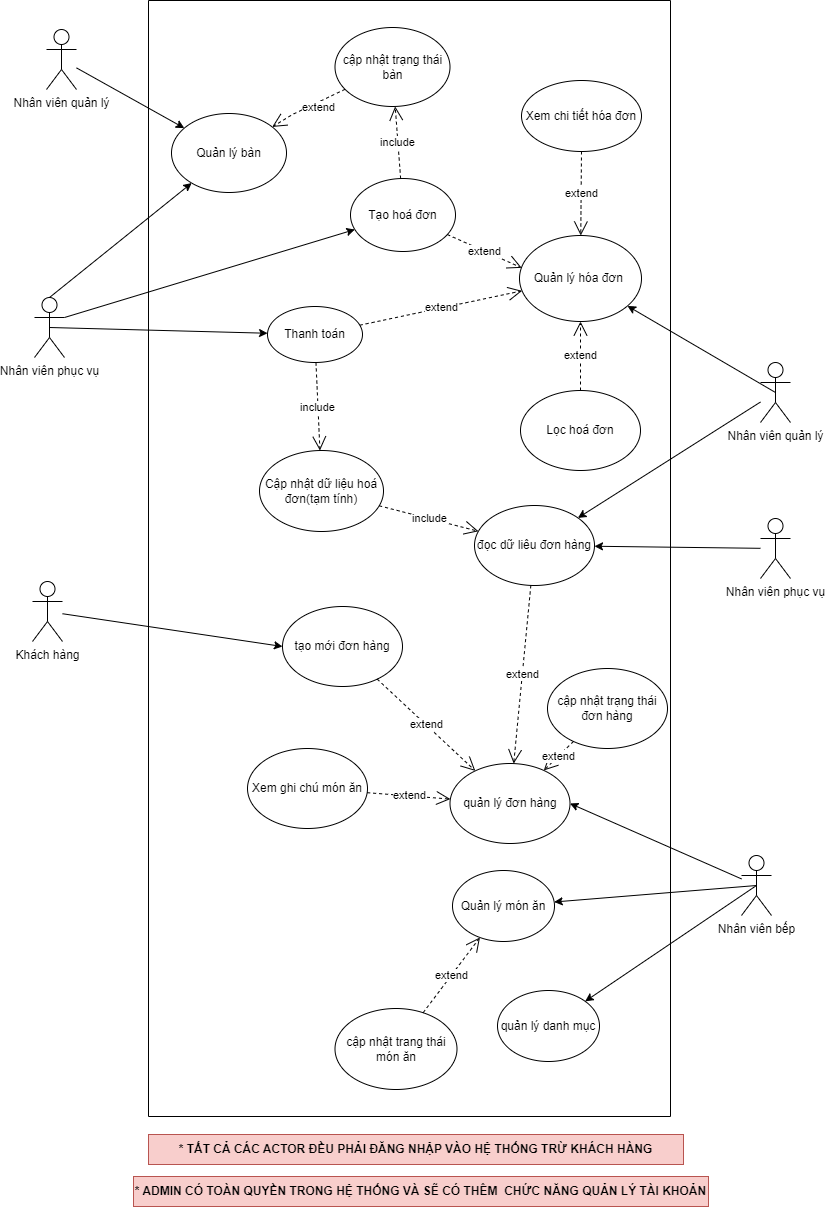
\includegraphics[scale=0.42]{img/usecase.png}
    	\caption{Sơ đồ Use Case}
    \end{center}
\end{figure}

\pagebreak

\section{Sơ đồ ERD}
\begin{figure}[htp]
    \begin{center}
    	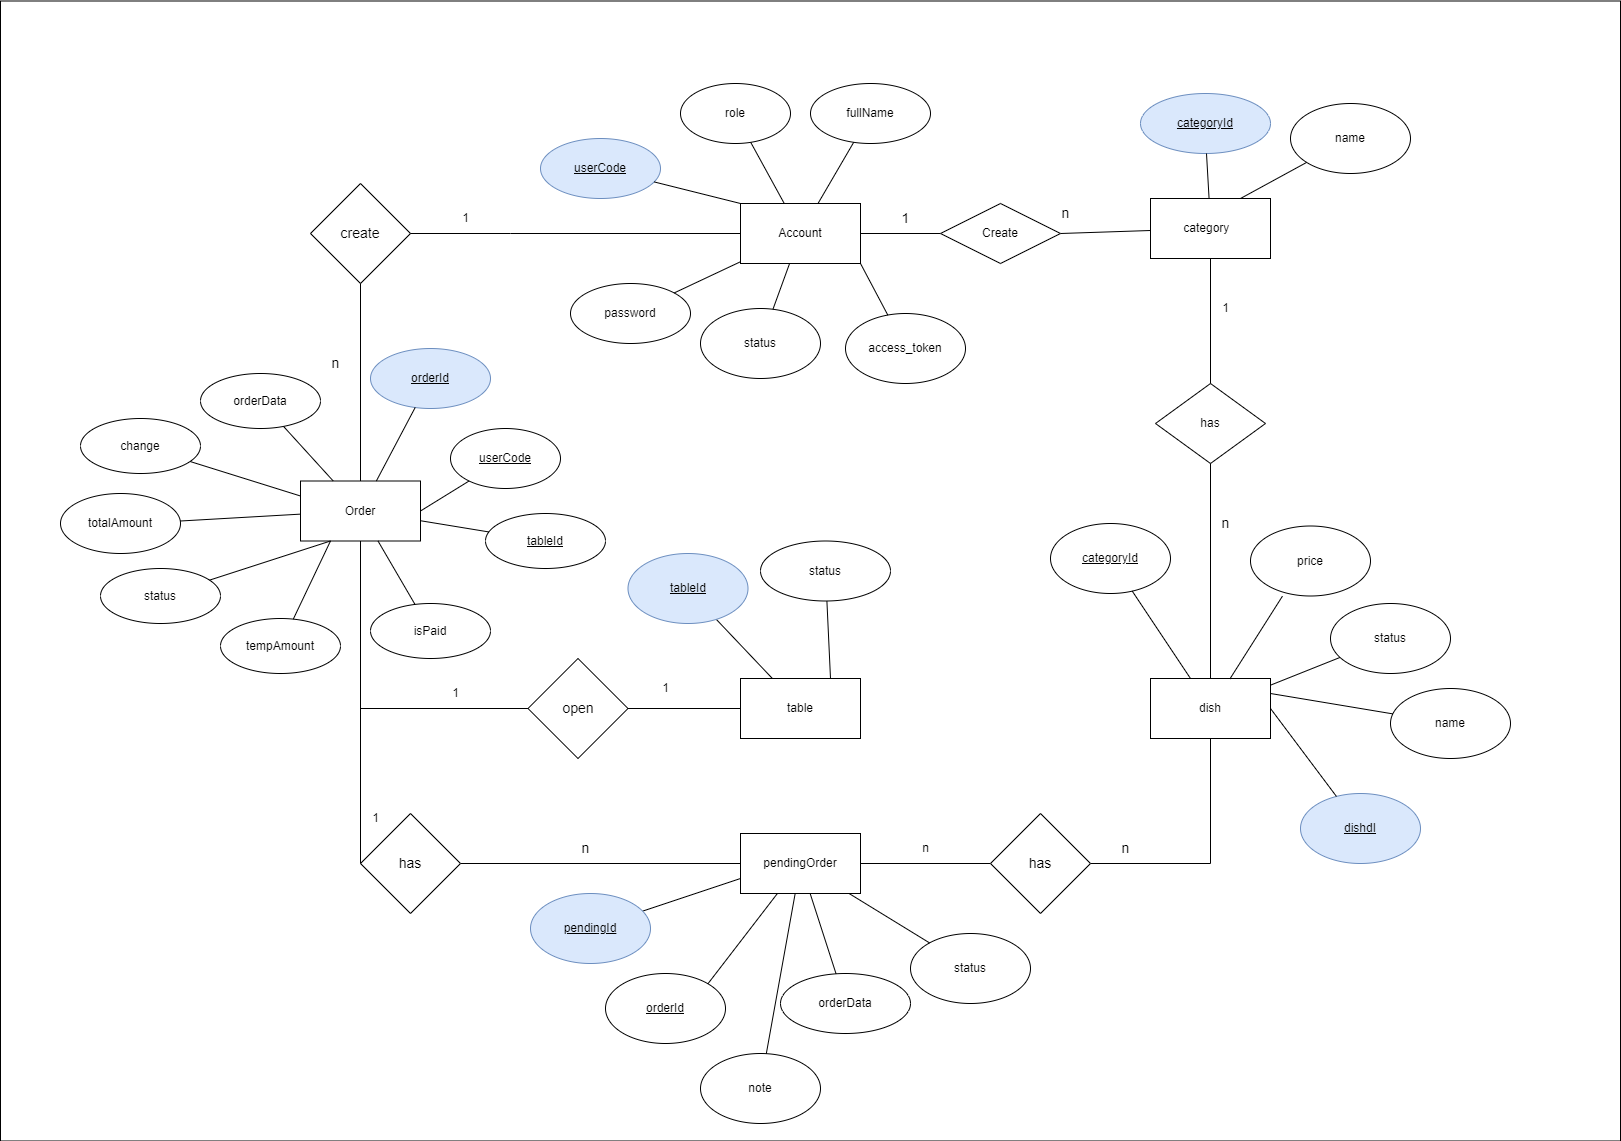
\includegraphics[width=\textwidth,height=\textheight,keepaspectratio]{img/erd_diagram.png}
    	\linebreak
    	\caption{Sơ đồ ERD}
    \end{center}
\end{figure}
\pagebreak

\section{Sơ đồ lớp}
\begin{figure}[H]
    \begin{center}
    	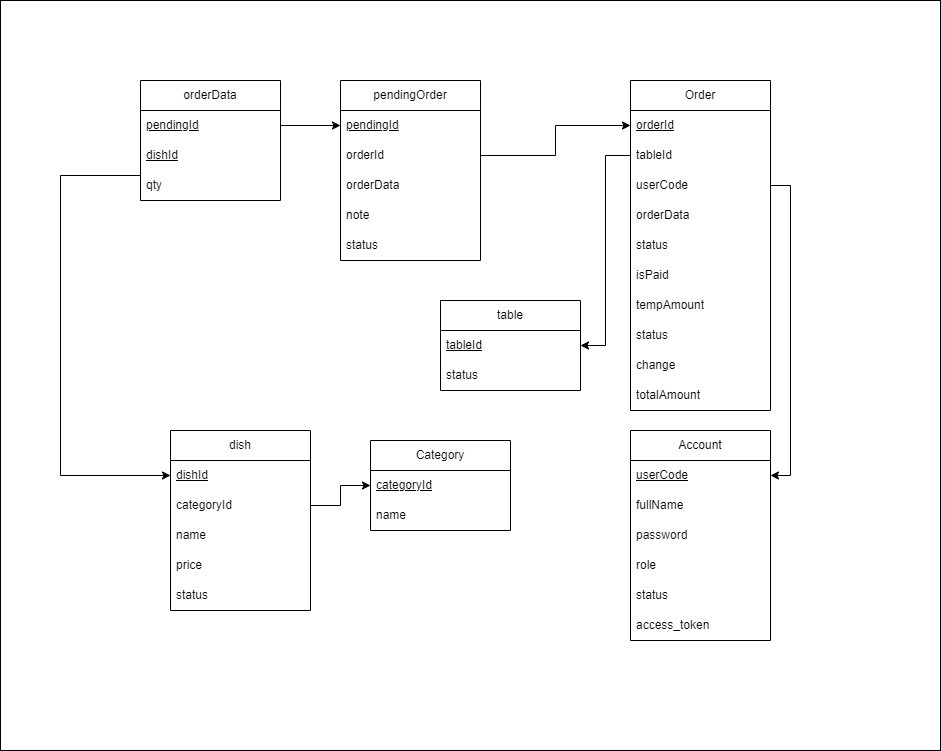
\includegraphics[width=\textwidth,height=\textheight,keepaspectratio]{img/class_diagram.png}
    	\linebreak
    	\caption{Sơ đồ lớp}
    \end{center}
\end{figure}


\chapter{Các chức năng (API) của phân hệ}
\section{Account}
\begin{figure}[H]
    \begin{center}
    	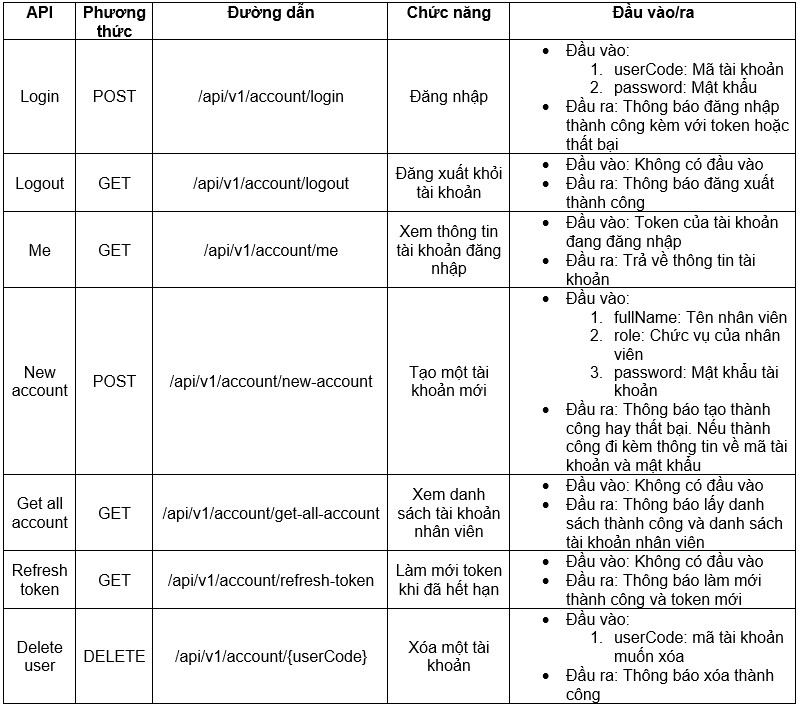
\includegraphics[width=\textwidth,height=\textheight,keepaspectratio]{img/API_Table_Account.jpg}
    	\linebreak
    	\caption{API của model Account}
    \end{center}
\end{figure}

\section{Category}

\begin{figure}[H]
    \begin{center}
    	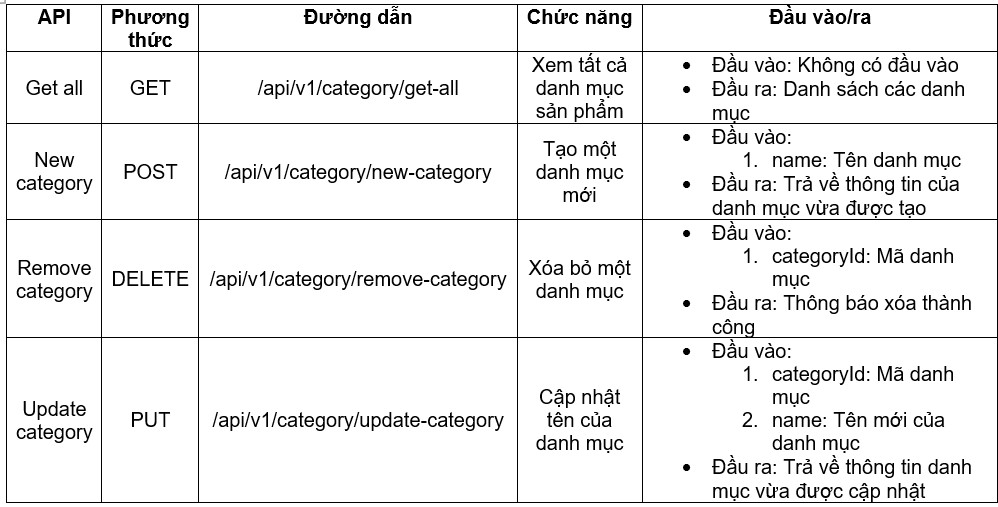
\includegraphics[width=\textwidth,height=\textheight,keepaspectratio]{img/API_Table_Category.jpg}
    	\linebreak
    	\caption{API của model Category}
    \end{center}
\end{figure}


\section{Order}

\begin{figure}[H]
    \begin{center}
    	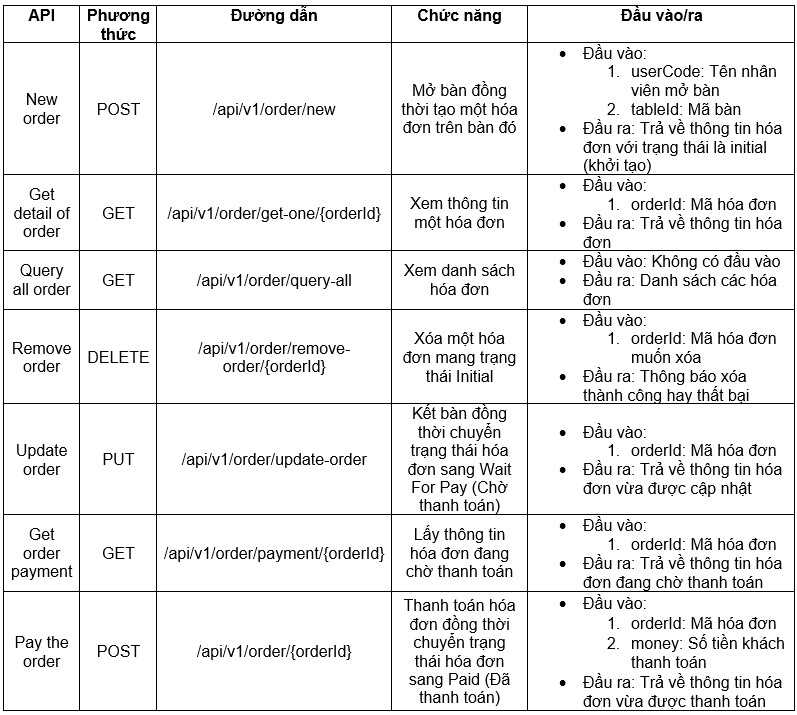
\includegraphics[width=\textwidth,height=\textheight,keepaspectratio]{img/API_Table_Order.jpg}
    	\linebreak
    	\caption{API của model Order}
    \end{center}
\end{figure}

\section{Pending Order}

\begin{figure}[H]
    \begin{center}
    	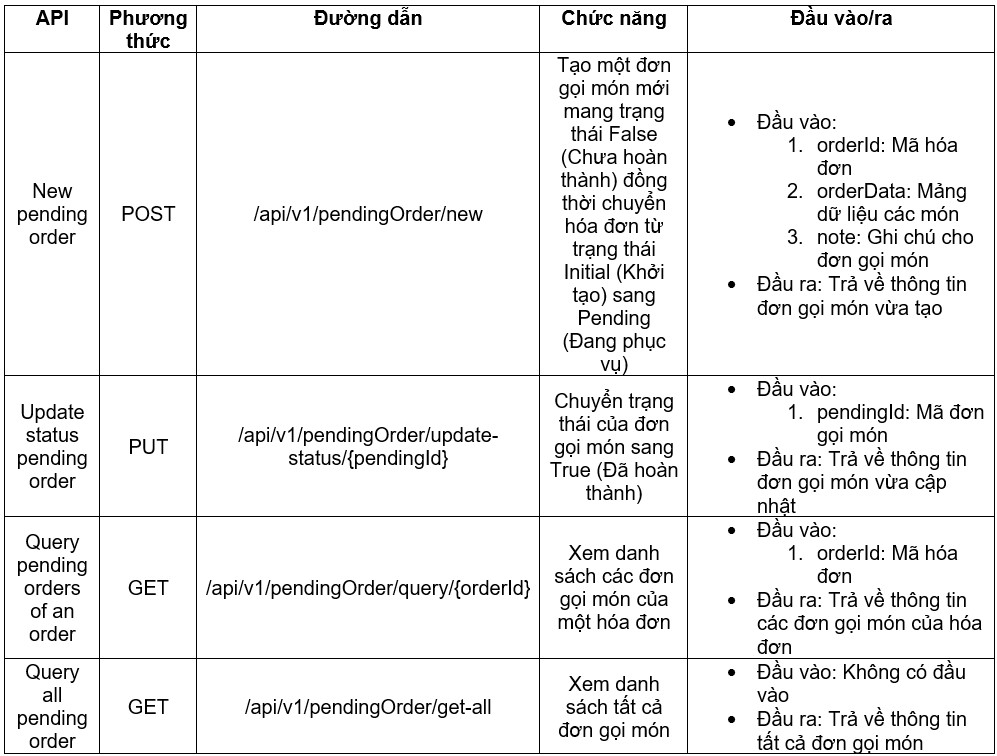
\includegraphics[width=\textwidth,height=\textheight,keepaspectratio]{img/API_Table_pendingOrder.jpg}
    	\linebreak
    	\caption{API của model pendingOrder}
    \end{center}
\end{figure}

\section{Table}

\begin{figure}[H]
    \begin{center}
    	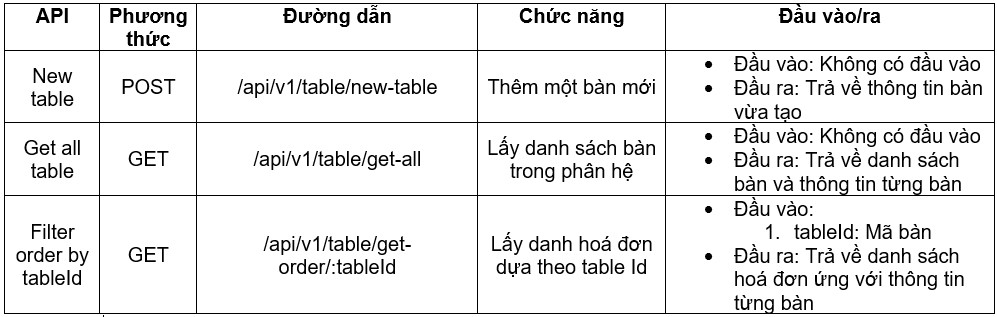
\includegraphics[width=\textwidth,height=\textheight,keepaspectratio]{img/API_Table_Table.jpg}
    	\linebreak
    	\caption{API của model Table}
    \end{center}
\end{figure}

\section{Dish}

\begin{figure}[H]
    \begin{center}
    	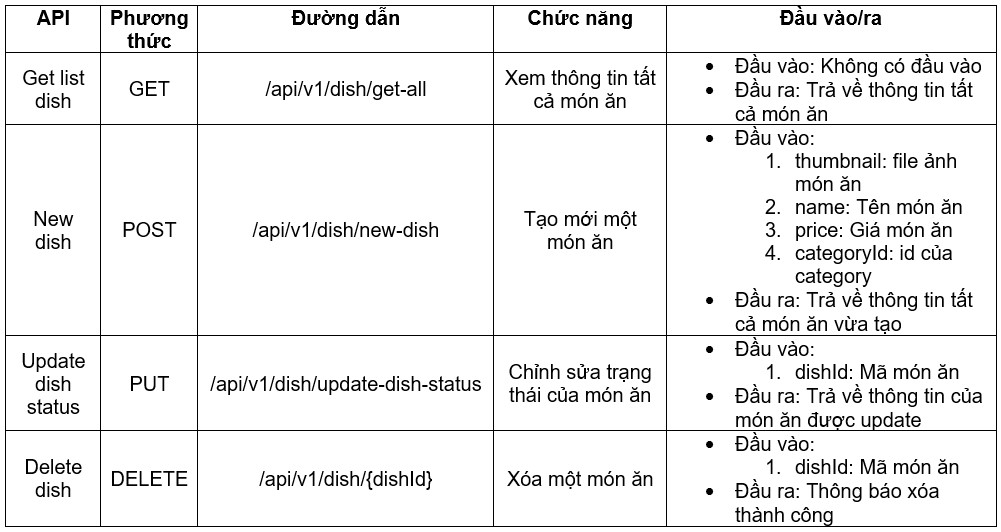
\includegraphics[width=\textwidth,height=\textheight,keepaspectratio]{img/API_Table_Dish.jpg}
    	\linebreak
    	\caption{API của model Dish}
    \end{center}
\end{figure}

\section{Menu}

\begin{figure}[H]
    \begin{center}
    	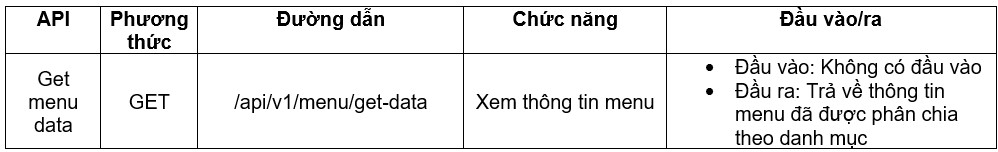
\includegraphics[width=\textwidth,height=\textheight,keepaspectratio]{img/API_Table_Menu.jpg}
    	\linebreak
    	\caption{API của model Menu}
    \end{center}
\end{figure}

\section{Invoice}

\begin{figure}[H]
    \begin{center}
    	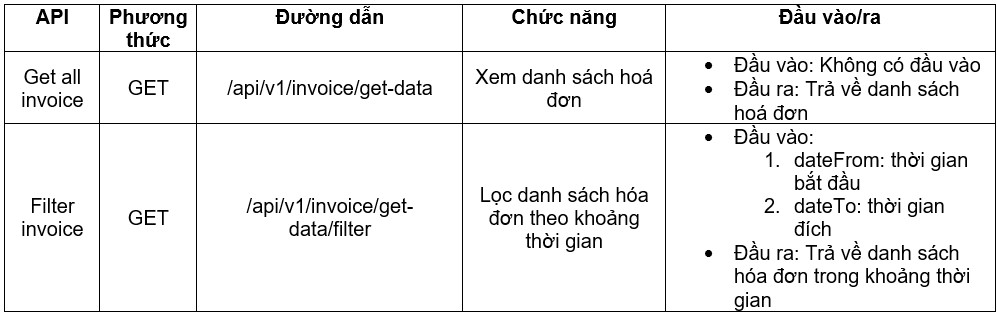
\includegraphics[width=\textwidth,height=\textheight,keepaspectratio]{img/API_Table_Invoice.jpg}
    	\linebreak
    \end{center}
\section{Demo api phân hệ (Swagger)}
\fontsize{15}{15}\selectfont
\paragraph{}
\end{figure}



\chapter{CÔNG NGHỆ SỬ DỤNG}
\begin{figure}[H]
\section{Express JS}
\fontsize{13}{15}\selectfont
	\paragraph{}
	Là một franework ứng dụng web back end để xây dựng các API RESTful với Node.js, được phát hành dưới dạng phần mềm mã nguồn mở và miễn phí theo Giấy phép MIT. Nó được thiết kế để xây dựng các ứng dụng web và API
	\paragraph{}	
	Vì Express js chỉ yêu cầu ngôn ngữ lập trình Javascript nên việc xây dựng các ứng dụng web và API trở nên đơn giản hơn với các lập trình viên và nhà phát triển.Expressjs cũng là một khuôn khổ của Node.js do đó hầu hết các mã code đã được viết sẵn cho các lập trình viên có thể làm việc.

\section{Vue JS}
\fontsize{13}{15}\selectfont
	\paragraph{}
	Là một framework linh động dùng để xây dựng giao diện người dùng (user interfaces - UI). Khác với các framework nguyên khối, Vue được thiết kế từ đầu theo hướng cho phép và khuyến khích việc phát triển ứng dụng theo các bước. Khi phát triển lớp giao diện, người dùng chỉ cần dùng thư viện lõi (core library) của Vue, vốn rất dễ học và tích hợp với các thư viện hoặc dự án có sẵn. Cùng lúc đó, nếu kết hợp với những kĩ thuật hiện đại như SFC (single file components) và các thư viện hỗ trợ, Vue cũng đáp ứng được dễ dàng nhu cầu xây dựng những ứng dụng đơn trang (SPA - Single Page Applications) với độ phức tạp cao.
	 \paragraph{}
	 Một ứng dụng Vue bao gồm một đối tượng Vue gốc. Ứng dụng này cũng thường được sắp xếp thành một cây gồm các component lồng nhau và tái sử dụng được
\end{figure}	
\begin{figure}[htp]
	\begin{center}
		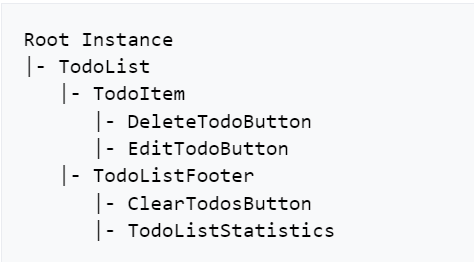
\includegraphics[scale=0.5]{img/vue_structure.png}		\linebreak
		\caption{Cây component của một ứng dụng todo sử dụng vue js}
	\end{center}
\end{figure}




\section{MongoDB}



\paragraph{}
MongoDB là một database hướng tài liệu (document), một dạng NoSQL database. Vì thế, MongoDB sẽ tránh cấu trúc table-based của relational database để thích ứng với các tài liệu như JSON có một schema rất linh hoạt gọi là BSON. MongoDB sử dụng lưu trữ dữ liệu dưới dạng Document JSON nên mỗi một collection sẽ các các kích cỡ và các document khác nhau. Các dữ liệu được lưu trữ trong document kiểu JSON nên truy vấn sẽ rất nhanh.
\FloatBarrier


\pagebreak



\begin{center}
	\pagenumbering{roman}\setcounter{page}{1}
	\fontsize{16}{20}\selectfont
	\textbf{TÀI LIỆU THAM KHẢO\\} 
\end{center}
\fontsize{16}{15}\selectfont
\section*{Link tham khảo}
\begin{enumerate}
\fontsize{13}{15}\selectfont
    \item Slide bài giảng
    \item \url{https://vuejs.org/}
    \item \url{https://nodejs.org/en/docs/guides} 
    \item \url{https://w3schools.com}
    \item \url{https://swagger.io}
    \item \url{https://www.npmjs.com/}
    \item \url{https://socket.io}
    \item \url{https://stackoverflow.com/}
    \item \url{https://chat.openai.com/}
\end{enumerate}
\end{document}
